\chapter{Analysis Tools}
\label{chap:analysis-tools}

\chapterquote{An architect's most useful tools are an eraser at the drafting board, and a wrecking bar at the site.}{Frank Lloyd Wright}

\section{Introduction}
Progressing from raw detector output to final results and distributions, which can be compared to theoretical predictions, involves a series of sequential steps.
The initial steps are generic to any analysis: the rejection of events for data quality reasons, the reconstruction of jets from calorimeter signals and their subsequent calibration are, in general, performed identically for each analysis.
Additionally, unfolding for detector effects, in other words correcting distributions made at detector level back to the final-state particle level, is
often necessary.

\section{Jet Reconstruction and Calibration}
\label{sec:analysis-tools:jet_reconstruction}
The default jet-clustering algorithm in \ATLAS is \akt (see \SectionRef{bg-theory:recombination_algorithms}), implemented using \fastjet~\cite{Cacciari:2005:fastjet,Cacciari:2012:fastjet}, with two different $R$-parameters: narrow jets with $R=0.4$ and wide jets with $R=0.6$.

Jets are reconstructed by applying a jet-clustering algorithm to calorimeter signals, and subsequently performing a calibration step, to correct for known detector effects.
Two different inputs from the calorimeter can be used for jet-finding, towers and topological clusters.

Towers are formed by collecting cells into bins of a regular $\DeltaEta \times \DeltaPhi = 0.1 \times 0.1$ grid, depending on their location, and summing up their signals, or a fraction of their signal corresponding to the overlap area fraction between the tower bin and the relevant cell.
This summing stage is non-discriminatory, in other words all calorimeter cells are used in the towers.
Towers with negative signals are recombined with nearby positive signal towers until the net signal is positive, thus all resulting towers have a valid physical four-vector and can directly be used by the jet finders.
This approach can be understood as an overall noise cancellation rather than suppression, since noisy cells will still contribute to the jets.

Topological cell clusters~\cite{ATLAS-LARG-PUB-2008-002} are an attempt to reconstruct three-dimensional energy depositions in the calorimeter~\cite{Cojocaru:2004:ATLASHadronicCalibration,Andrieu:1993:H1PionCalibration}.
Firstly, any cell which satisfies $|E_{cell} | > 4\sigma_{cell}$ is identified as a ``seed cell'', where $\sigma$ is the RMS noise of the cell due to electronic effects and pile-up.
Any cell neighbouring a seed cell, which itself satisfies $|E_{cell}| > 2\sigma_{cell}$, is incorporated into the topocluster, and this process is repeated iteratively until there are no longer any cells adjacent to the topocluster with $|E_{cell}| > 2\sigma_{cell}$.
Finally, an outer layer of cells is added, here accepting any surrounding cells which satisfy $E_{cell} > 0$ is added.
Known hot cells or dead cells are excluded from this process.
In contrast to using signal towers, using this 4-2-0 clustering scheme inherently incorporates noise suppression and results in fewer cells being included in the jet clustering step.
In jet reconstruction, each topocluster is considered to be a massless particle with energy $E = \sum{E_{cell}}$ and position given by the energy-weighted centroid of cells in the cluster, with the direction pointing back towards the geometric centre of the detector.

Jets produced in this way are reconstructed at the electromagnetic (EM) scale, which is the basic signal scale for the \ATLAS calorimeters. It accounts
correctly for the energy deposited in the calorimeter by electromagnetic showers - validated using test-beam measurements with electrons and muons.
It does not, however, correct for the lower hadron response, and a series of calibration steps is therefore needed to bring an uncalibrated, EM-scale jet to the hadronic scale energy scale~\cite{ATLAS-CONF-2010-056,CERN-PH-EP-2011-191}.
Jets which fall below the reconstruction threshold of \unit{7}{\GeV} are discarded before calibration.

\subsection{Pile-up Correction}
\label{sec:analysis-tools:pileup_correction}
Jets calibrated at the EM-scale are affected by energy deposits arising from multiple proton-proton interactions within the same bunch crossing, known as
pile-up.
Pile-up can be either out-of-time, in other words, occurring slightly before or after the hard interaction or in-time, occurring contemporaneously.
The \ATLAS calorimeter response is such that the time integral of the signal corresponding to a single particle is zero: in other words a sharp positive peak is followed by a longer but lower amplitude trough.
This ensures that the calorimeter is not saturated when large numbers of particles arrive in close succession but also means that, while in-time pile-up provides a positive contribution to the calorimeter signal, out-of-time pile-up will provide negative contribution.
A correction to remove the average effects of these additional proton-proton interactions, derived using minimum bias data, is applied at the electromagnetic scale: the average additional \ET per calorimeter tower, measured as a function of \pseudorap and the number of reconstructed primary vertices $N_{PV}$, is subtracted from each jet.

\subsection{Jet Origin Correction}
The calorimeter clusters used for jet reconstruction are assumed to originate from the geometrical centre of ATLAS.
The jet origin correction first corrects each calorimeter cluster to instead point back to the primary vertex with the highest $\sum{\pT^{track}}$ of the event; the beam spot is used if there is no primary vertex.

The kinematics of each calorimeter cluster are recalculated using the direction from the primary vertex to the centroid of the cluster.
The raw jet four momentum is then redefined as the four vector sum of the clusters.
This correction improves the angular resolution while the jet energy is unaffected.
A small improvement in jet \pT resolution is introduced due to the changing jet direction, although this is rarely larger than 1\%.
Most of the effect of the correction comes from the $z$-position of the primary vertex.

\subsection{Final Jet Energy Scale}
\label{sec:analysis-tools:final_JES}
The final part of the jet calibration involves applying a jet energy scale (JES) correction to account for the fact that the jets are reconstructed at the
electromagnetic (EM) scale.
This is known as the EM+JES calibration, and it corrects for  calorimeter non-compensation, energy losses in inactive regions, out-of-cone showering effects as well as inefficiencies in the calorimeter clustering and jet reconstruction.
This calibration is primarily dependent on energy, since the calorimeter response is energy-dependent, and the jet direction, due to the changing calorimeter technology and to the varying amounts of dead material in front of the calorimeters.

The EM+JES calibration is derived from simulated events, specifically the AMBT1 \Pythia \dijet sample.
To derive the correction factors in \MC, isolated particle jets, reconstructed using final-state particles, are matched with isolated detector level jets, reconstructed using the full calorimeter level information.
The particle jet energy is then divided by the EM-scale energy of the matching calorimeter jet in order to obtain the appropriate correction factor.

Following this, a small \pseudorap-dependent correction is applied to remove a bias in the reconstructed \pseudorap of jets that occurs when jets fall in poorly instrumented regions of the calorimeter that have a lower response than the regions around it.
The reconstructed direction of the jet will be biased since the clusters that fall in these regions have a lower response when their four-vectors are added up to build the jet four-vector, and hence a smaller overall weight.
As a consequence of this, the jet is pulled toward the region with the higher response.
This \pseudorap-correction is parameterized as a function of jet energy and pseudorapidity, and is small, $\DeltaEta < 0.01$, in most regions of the calorimeter, although larger in the crack regions: up to $\DeltaEta = 0.07$ for low \pT jets in the HEC-FCAL transition region.

\section{Generic Event Selection Considerations}
\label{sec:analysis-tools:data_selection}
\subsection{Luminosity}
All of the studies presented in this thesis were carried out at a centre-of-mass
energy of \rootS = \unit{7}{\TeV} using the \twentytenlumi of integrated
luminosity that was collected during 2010 (see \FigureRef{fig:analysis-tools:luminosity}).

The luminosity was measured independently by multiple detectors and algorithms,
each of which had differing acceptances, systematic uncertainties and background 
sensitivities. In 2010, the primary methods used were LUCID, a dedicated \v{C}erenkov
detector and counting hits in the MBTS. For both of these, the case in which hits
were registered on the A-side AND the C-side of the detector was treated as a separate
measurement from the case in which the requirement was only for a hit on at least
one of these.

\begin{figure}[htpb]
  \subfloat[2010 luminosity evolution]{
    \includegraphics[width=\smallfigwidth]{chapters/analysis-tools/sum2010LumiByDay.eps}
    \label{fig:analysis-tools:luminosity_nonLog}}
  \quad
  \subfloat[2010 luminosity evolution, logarithmic scale]{
    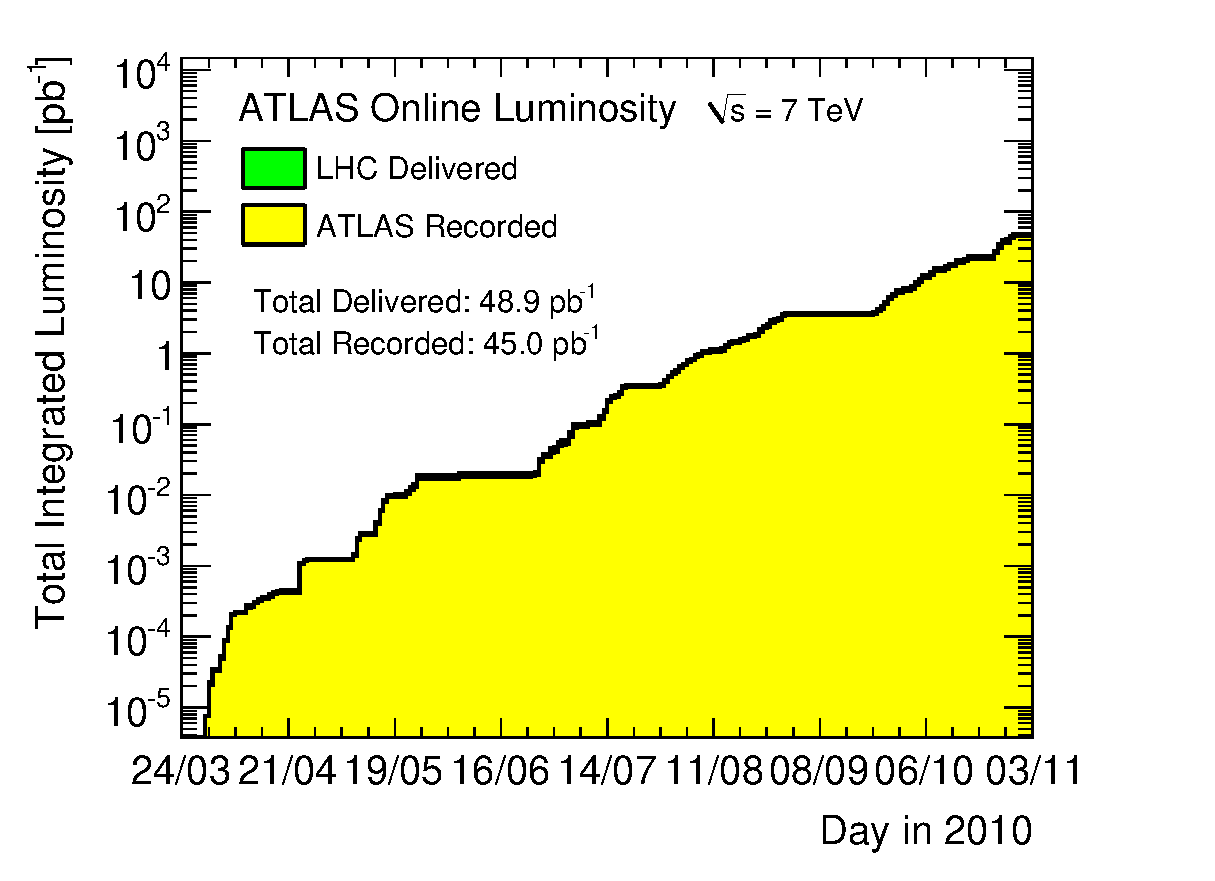
\includegraphics[width=\smallfigwidth]{chapters/analysis-tools/sum2010LumiByDayLog.eps}
    \label{fig:analysis-tools:luminosity_log}}
  \caption{Total integrated luminosity available in \ATLAS and recorded by the \LHC in 2010. Identical information is shown in \protect\subref{fig:analysis-tools:luminosity_nonLog} and \protect\subref{fig:analysis-tools:luminosity_log}, with the only difference being that a logarithmic scale is used in the latter case~\cite{ATLAS-CONF-2011-011}.}
  \label{fig:analysis-tools:luminosity}
\end{figure}

The van der Meer method discussed in \SectionRef{sec:bg-theory:luminosity} was used
to obtain $\sigma_{vis}$ for each of these processes. The differences between the
luminosities obtained from each method were monitored as a function of time
and of $\mu$. The measurements were finally combined to produce the overall \ATLAS
luminosity determination, together with its uncertainty~\cite{CERN-PH-EP-2010-069}.

A single run of proton-proton collisions is divided into luminosity blocks, each of
which typically represents about two minutes of data taking, within which
conditions such as bunch spacing and beam intensity are constant. The
instantaneous luminosity, bunch size and bunch shaping each evolved over the
course of this period of data taking; data collected in \ATLAS is therefore divided
into different run periods, with the boundaries of these periods being defined by
changes in running conditions. The dates and total integrated luminosity corresponding
to each of these run periods are summarised in \TableRef{tab:analysis-tools:luminosity-periods}.

\begin{table}
\begin{center}
  \begin{tabular}{ c@{\hskip 1cm} c c c c c }
    Period                         &   A    &   B    &   C    &   D    &   E    \\
    Start of data taking           & Mar 30 & Apr 23 & May 18 & Jun 24 & Jul 29 \\
    End of data taking             & Apr 19 & May 17 & Jun 05 & Jul 18 & Aug 17 \\
    Luminosity [$\nano\barn^{-1}$] & 0.380  & 8.07   & 8.46   & 201    & 1000   \\
    \cmidrule{2-6}
    Period                         &   E5   &   F    &   G    &   H    &  I     \\
    Start of data taking           & Aug 10 & Aug 19 & Sep 22 & Oct 08 & Oct 24 \\
    End of data taking             & Aug 17 & Aug 30 & Oct 06 & Oct 18 & Oct 29 \\
    Luminosity [$\nano\barn^{-1}$] & 445    & 1810   & 6870   & 7250   & 19100  \\
  \end{tabular}
  \caption{Dates and total integrated luminosity for each of the nine data taking periods for data collected by \ATLAS in 2010. Separate numbers are presented for period E and period E5 (which excludes the first four sets of runs in this period) due to a software problem which affected forward jet triggers at this time.}
  \label{tab:analysis-tools:luminosity-periods}
\end{center}
\end{table}

\subsection{Data Quality}
Certain generic cuts, held in common between all analyses are necessary in order
to extract useful events from the recorded data. First, the event is required to
belong to one of a set of ``good runs''. These are specific luminosity blocks in
which the relevant detector subsystems, trigger and reconstructed physics
objects have passed a data-quality assessment and are deemed suitable for
physics analysis. For the analyses discussed in this thesis, this means the
central trigger processor, solenoid magnet, inner detectors (Pixel, SCT, and
TRT), calorimeters (barrel, end-cap, and forward) and the luminosity recording
system.

\subsection{Primary Vertex}
To reject events arising from cosmic-ray muons and other non-collision backgrounds,
events are selected as collision candidates by requiring that they have at
least one primary vertex that is consistent with the beamspot position and that
has at least five tracks associated to it, each with $\pT > \unit{0.5}{\GeV}$.
This vertex definition is consistent with that used to evaluate pile-up vertices
in the offset correction, as discussed in \SectionRef{sec:analysis-tools:pileup_correction}.
The efficiency for collision events to pass this vertex requirement, although
obviously analysis dependent, is generally well over 99\%.

\subsection{Jet Cleaning}
\label{sec:analysis-tools:jet_cleaning}
Standard jet cleaning criteria have been developed in order to identify fake jets
which arise due to noise or to out-of-time energy depositions. Jets failing these criteria
are flagged as either ``bad'', likely to be fake, or ``ugly'', likely to be
mismeasured due to falling into less well instrumented
regions~\cite{ATLAS-CONF-2010-038,ATLAS-CONF-2010-050}. Three main issues are
addressed, with a dedicated set of selection criteria for each:

\begin{itemize}
  \item \textbf{Single-cell jets in the HEC.} Most misreconstructed jets arise
    from noise bursts in the HEC. This results in jets with most of their energy
    coming from single calorimeter cells.
  \item \textbf{Bad quality jets in the EM calorimeter.} Noise bursts in the
    EM calorimeter, although rarer than in the HEC, result in jets with most of
    their energy coming from the EM calorimeter and whose cells have bad
    reconstruction ``quality\footnote{$Q$-factor, one of the inputs to jet cleaning,
                                      is a measure of the quality of the signal
                                      in a given LAr cell, analogous to $\chi^2$,
                                      parameterising how well the expected pulse
                                      shape fits the digitised samples and thus
                                      how well the amplitude is measured in this
                                      cell. Cutting on this variable aims to remove
                                      large but badly measured cell amplitudes which
                                      could otherwise fake a jet.}''.
  \item \textbf{Out-of-time jets.} When large out-of-time energy deposits appear
    in the calorimeter, possibly from photons produced by cosmic rays, jets will
    be reconstructed with timing that is incompatible with the event time.
\end{itemize}

A series of per-jet variables, seen in \TableRef{tab:analysis-tools:jet_cleaning_variables}
are used to reject jets falling into one of these categories.

\begin{table}
\begin{center}
  \begin{tabular}{ c l }
  EMf        & fraction of energy coming from the EM calorimeter                             \\
  FMax       & maximum energy fraction in one calorimeter layer                              \\
  HECf       & energy fraction in the HEC                                                    \\
  LArQ       & the fraction of energy coming from LAr cells having $Q$-factor $>4000$        \\
  HECQ       & same as the LArQuality except calculated only with the HEC                    \\
  NegE       & negative energy in the jet                                                    \\
  t          & the mean timing difference between cells in the jet and the event time        \\
  \pseudorap & \pseudorap at the EM-scale                                                    \\
  Chf        & the ratio of the $\sum{\pT^{track}}$ associated to the jet divided by jet \pT \\
  \end{tabular}
  \caption{Per-jet variables used as an input to jet cleaning.}
  \label{tab:analysis-tools:jet_cleaning_variables}
\end{center}
\end{table}

Three levels of bad jet rejection have been determined by the \ATLAS Jet/Etmiss
Working Group. The most lenient of these is termed ``loose'' cleaning, with
``medium'' and ``tight'' successively applying stricter criteria in identifying
additional jets as bad. The jet cleaning cuts used in each of these cases are
shown in \TableRef{tab:analysis-tools:jet_cleaning}.

\begin{table}
\begin{center}
  \begin{tabular}{ l c c c }
             & Loose                            & Medium = Loose OR             & Tight = Medium OR     \\ 
  \midrule
             & $\text{HECf}>0.5$ \&             &                               &                       \\
  HEC        & $|\text{HECQ}|>0.5$              & $\text{HECf}>1-|\text{HECQ}|$ &                       \\
  spikes     & OR                               &                               &                       \\
             & $|\text{NegE}|>\unit{60}{\GeV}$  &                               &                       \\
  \midrule
             & $\text{EMf}>0.95$ \&             & $\text{EMf}>0.9$ \&           &  $\text{EMf}>0.98$ \& \\
  EM         & $|\text{LArQ}|>0.8$ \&           & $|\text{LArQ}|>0.8$ \&        & $|\text{LArQ}|>0.05$  \\
  coherent   & $|\eta|<2.8$                     & $|\eta|<2.8$                  &                       \\
  noise      &                                  &                               & OR                    \\
             &                                  &                               & $|\text{LArQ}|>0.95$  \\
  \midrule
             & $|t|<\unit{25}{\nano\second}$    & $|t|<\unit{10}{\nano\second}$ &                       \\
             & OR                               & OR                            &                       \\
             & $\text{EMf}<0.05$ \&             & $\text{EMf}<0.05$ \&          & $\text{EMf}<0.1$ \&   \\
  Non-       & $\text{Chf}<0.05$ \&             & $\text{Chf}<0.1$ \&           & $\text{Chf}<0.2$ \&   \\
  collision  & $|\eta|<2$                       & $|\eta|<2$                    & $|\eta|<2$            \\
  background & OR                               & OR                            & OR                    \\
  and        & $\text{EMf}<0.05$ \&             & $\text{EMf}>0.95$ \&          & $\text{EMf}>0.9$ \&   \\
  cosmics    & $|\eta| \geq 2$                  & $\text{Chf}<0.05$ \&          & $\text{Chf}<0.02$ \&  \\
             &                                  & $|\eta|<2$                    & $|\eta|<2$            \\
             & OR                               &                               &                       \\
             & $\text{FMax}>0.99$ \&            &                               & $\text{EMf}<0.1$ \&   \\
             & $|\eta|<2$                       &                               & $|\eta| \geq 2$       \\
  \end{tabular}
  \caption{The cuts used to remove bad jets as part of jet cleaning in \ATLAS.
           Each of the three sets of cuts are shown: loose, medium and tight. A
           jet is considered ``bad'' if it passes any of these cuts. The medium
           cuts comprise the loose cuts plus additional requirements, while the
           tight cuts have the same relationship to the medium cuts. This means
           that any jet considered bad by the loose (medium) cuts will
           automatically be considered bad when using the medium (tight) cuts.}
  \label{tab:analysis-tools:jet_cleaning}
\end{center}
\end{table}

As well as this removal of bad jets, ugly jets are identified as those jets
with more than 50\% of their energy coming either from TileGap3, the transition
region between the barrel and end-cap, or from known dead cells, which are
assigned an energy value based on the values of their neighbouring cells.

\subsection{Jet Energy Scale Uncertainty}
\label{sec:analysis-tools:jes_uncertainty}
As discussed in \SectionRef{sec:analysis-tools:final_JES}, the jet energy scale
(JES) is derived in \MC before being validated using a series of in-situ
measurements. Evaluating the JES uncertainty therefore necessitates combining
uncertainties arising from each of these sources: in-situ and single pion
test-beam measurements, uncertainties on precise details of material
distribution in the \ATLAS detector, the \MC modelling used in event simulation
and electronic noise must all be considered~\cite{ATLAS-CONF-2010-056,CERN-PH-EP-2011-191}.
%The jet energy scale (JES), as discussed in ,
%has multiple sources of systematic uncertainty, Evaluation of the level of
%uncertainty on the JES requires information from each of these sources to be combined:

Important individual sources of uncertainty include: non-closure when the JES
correction is applied to reconstructed \MC; the single particle calorimeter response determined
from in-situ measurements, as described in \SectionRef{sec:detector:single-particle};
the accuracy of detector simulations obtained by varying calorimeter noise in \MC samples; the
uncertainty associated with physics modelling, which is obtained from comparing
the detector response in different \MC generators and finally the  relative
jet calibration obtained through \etaint, as discussed in
\ChapterRef{chap:eta-intercalibration}. The level of JES uncertainty is shown in
\FigureRef{fig:analysis-tools:JESUncertainty} as a function of jet \pT for
central and for forward jets.

\begin{figure}[htpb]
  \subfloat[$0.3 \leq \absEta < 0.8$]{
    \includegraphics[width=\smallfigwidth]{chapters/analysis-tools/JESUncertainty_AntiKt6Topo_EMJES0.3-0.8.eps}
    \label{fig:analysis-tools:JESUncertainty_central}}
  \quad
  \subfloat[$3.6 \leq \absEta < 4.5$]{
    \includegraphics[width=\smallfigwidth]{chapters/analysis-tools/JESUncertainty_AntiKt6Topo_EMJES3.6-4.5.eps}
    \label{fig:analysis-tools:JESUncertainty_forward}}
  \caption{Fractional jet energy scale systematic uncertainty is shown as a
           function of \pT for jets in two pseudorapidity regions: \protect\subref{fig:analysis-tools:JESUncertainty_central}
           $0.3 \leq \absEta < 0.8$ and \protect\subref{fig:analysis-tools:JESUncertainty_forward}
           $3.6 \leq \absEta < 4.5$. In the forward region, the JES uncertainty
           is extrapolated from the barrel uncertainty, with the uncertainty contribution
           from the \etaint between central and forward jets in data and \MC added
           in quadrature. The total uncertainty is shown as the solid light blue
           area. The individual sources are also shown, with uncertainties from
           the fitting procedure where applicable~\cite{ATLAS-CONF-2010-056,CERN-PH-EP-2011-191}.}
  \label{fig:analysis-tools:JESUncertainty}
\end{figure}

\subsection{Jet Trigger Threshold Evolution}
\label{sec:analysis-tools:jet_selection_evolution}
As data conditions have changed over time, the trigger has changed to reflect
this: both through enabling the HLT, which was initially used in passthrough
mode, and by changing trigger prescales to keep the overall recorded event rate
within acceptable bounds. This was primarily done by prescaling triggers with
lower \ET thresholds, while the triggers with the highest \ET thresholds
remained unprescaled.

In general, the aim of jet-based analyses is to retain as high a proportion of events as
possible while minimising the biases and systematic uncertainties arising from
the trigger. The easiest way to achieve this is to use the trigger in the
plateau region where its efficiency is close to 100\%. In order to accept as
many events as possible, hence reducing statistical uncertainty, the trigger
thresholds used in analyses are usually chosen to be the lowest ones for which
trigger efficiency is still larger than 99\%, thus ensuring that the effects of
prescaling are as small as possible.

For high \pT jets in the central region, this means that the trigger of choice
changes over time, as successive triggers become increasingly prescaled. For
low \pT jets, the majority of the recorded data comes from periods A--C, recorded
between March and June 2010, when much of the trigger bandwidth was allocated to
minimum bias triggers. For forward jets, the first four periods (A--D) could not
be used, as the forward jet trigger had not yet been commissioned, so the
majority of analyses can use only periods E--I.

In 2010 only L1 information was used to select events in the early periods, up
until the summer, while L2 was used from the summer to the end of the year. The
jet trigger did not reject events at the EF stage in 2010. In the early part of
Period A, before run 152777, a mistiming in the L1 central jet trigger hardware
caused large inefficiencies although MBTS triggers were not affected by this.
Additionally, further calibration problems mean that forward jet triggers cannot
be used during the early runs of period E.

\section{Unfolding Detector Effects}
\label{sec:analysis-tools:unfolding}
Unfolding is a procedure which attempts to correct distributions made using
information from the detector output back to the equivalent distributions that
would have been seen given an ideal detector which was able to perfectly measure
all final-state particles in the event. Unfolding aims to compensate for
smearing effects in the detector as well as for event selection inefficiencies. This
allows easy comparison to any theoretical calculation even if, at some future
point, the precise details of the detector simulation are lost.

Various different unfolding methods are used in different analyses, but they all
share one essential feature: they rely on comparison, using one or more \MC{s}
generators, between final-state particle level (hadron level) information and
the equivalent information after detector simulation and reconstruction have
been applied (detector level).

Bin-by-bin unfolding relies entirely on the shape of distributions in \MC in order
to compute the correction factors. Firstly, for each relevant distribution, the
ratio between the hadron level and detector level predictions is calculated.
This ratio is then applied as a correction factor to the measured data. This
technique can only be applied when migrations between bins are small in
comparison to the bin contents, often forcing the use of large bins. Efficiency,
the proportion of events which remain in the same bin between hadron level and
detector level, and purity, the proportion of events in a given detector level
bin which were in that bin at hadron level are important in assessing the impact
of inter-bin migrations.

For the Singular Value Decomposition (SVD) method, the first step is to
construct a 2D transfer matrix, providing full information about movements from
one bin to another between hadron level and detector level. A singular value
decomposition is then used in order to prevent fluctuations that a simple
inversion of this transfer matrix would introduce. However, the regularisation
procedure in SVD also uses a constraint on the curvature of the unfolded
spectrum, which introduces long-range correlations in the result that produce an
artificial smoothing of the unfolded distribution and which can also cause
biases.

The Iterative, Dynamically Stabilised (IDS) method uses the same transfer matrix
to compute the matrix of unfolding probabilities, which encodes the probability
for an event reconstructed in a given bin $i$ to be generated in bin $j$. The
unfolding matrix is improved in a series of iterations, where the hadron level \MC is
reweighted to the shape of the corrected data spectrum. The regularisation,
preventing statistical fluctuations from being amplified by the successive
iterations, is provided by the use of the significance of the differences
between data and \MC in each bin. The final unfolding matrix, after the optimal
number of iterations, is used to correct the reconstructed spectrum for detector
effects.

Finally, unfolding based on Bayes' theorem uses the transfer matrix to obtain a
series of transition probabilities: given a certain hadron level result, what are
the probabilities for each detector level measured outcome. Bayes' theorem is then
used to calculate the reverse probability: given a detector level outcome, what
is the probability that the hadron level result could have come from each bin of
the measurement: this process is then repeated iteratively~\cite{DAgostini:2010:BayesianUnfolding}.
